
\documentclass{article}
\usepackage{amsfonts}

%%%%%%%%%%%%%%%%%%%%%%%%%%%%%%%%%%%%%%%%%%%%%%%%%%%%%%%%%%%%%%%%%%%%%%%%%%%%%%%%%%%%%%%%%%%%%%%%%%%
\usepackage{amsmath}

%TCIDATA{OutputFilter=LATEX.DLL}
%TCIDATA{Created=Tuesday, August 12, 2003 11:49:27}
%TCIDATA{LastRevised=Monday, September 29, 2003 10:30:46}
%TCIDATA{<META NAME="GraphicsSave" CONTENT="32">}
%TCIDATA{<META NAME="DocumentShell" CONTENT="Articles\SW\Standard LaTeX Article">}
%TCIDATA{CSTFile=LaTeX article (bright).cst}

\newtheorem{theorem}{Theorem}
\newtheorem{acknowledgement}[theorem]{Acknowledgement}
\newtheorem{algorithm}[theorem]{Algorithm}
\newtheorem{axiom}[theorem]{Axiom}
\newtheorem{case}[theorem]{Case}
\newtheorem{claim}[theorem]{Claim}
\newtheorem{conclusion}[theorem]{Conclusion}
\newtheorem{condition}[theorem]{Condition}
\newtheorem{conjecture}[theorem]{Conjecture}
\newtheorem{corollary}[theorem]{Corollary}
\newtheorem{criterion}[theorem]{Criterion}
\newtheorem{definition}[theorem]{Definition}
\newtheorem{example}[theorem]{Example}
\newtheorem{exercise}[theorem]{Exercise}
\newtheorem{lemma}[theorem]{Lemma}
\newtheorem{notation}[theorem]{Notation}
\newtheorem{problem}[theorem]{Problem}
\newtheorem{proposition}[theorem]{Proposition}
\newtheorem{remark}[theorem]{Remark}
\newtheorem{solution}[theorem]{Solution}
\newtheorem{summary}[theorem]{Summary}
\newenvironment{proof}[1][Proof]{\textbf{#1.} }{\ \rule{0.5em}{0.5em}}
\input{tcilatex}

\begin{document}

\title{The Title of a Standard LaTeX Article}
\author{A. U. Thor \\
%EndAName
The University of Stewart Island}
\maketitle

\begin{abstract}
We study the effects of warm water on the local penguin population. The
major finding is that it is extremely difficult to induce penguins to drink
warm water. The success factor is approximately $-e^{-i\pi }-1$.
\end{abstract}

\begin{enumerate}
\item Inverso \FRAME{dtbpFU}{3in}{2.0003in}{0pt}{\Qcb{$m\in \gz^{-}$}}{}{Plot%
}{\special{language "Scientific Word";type "MAPLEPLOT";width 3in;height
2.0003in;depth 0pt;display "PICT";plot_snapshots TRUE;mustRecompute
FALSE;lastEngine "Maple";xmin "-5";xmax "5";xviewmin "0.01";xviewmax
"5.000000";yviewmin "0.001";yviewmax "5.000";viewset"XY";plottype
4;numpoints 49;plotstyle "patch";axesstyle "normal";xis \TEXUX{x};yis
\TEXUX{y};var1name \TEXUX{$x$};var2name \TEXUX{$y$};function
\TEXUX{$x^{-1}$};linecolor "black";linestyle 1;pointstyle
"point";linethickness 3;lineAttributes "Solid";var1range
"-5,5";num-x-gridlines 49;curveColor "[flat::RGB:0000000000]";curveStyle
"Line";rangeset"X";valid_file "T";tempfilename
'HJIMTF0G.wmf';tempfile-properties "XPR";}}

\item Directamente proporcional \FRAME{dhFU}{3in}{2.0003in}{0pt}{\Qcb{$m=1\
\ y=mx$}}{}{Plot}{\special{language "Scientific Word";type "MAPLEPLOT";width
3in;height 2.0003in;depth 0pt;display "PICT";plot_snapshots
TRUE;mustRecompute FALSE;lastEngine "Maple";xmin "-5";xmax "5";xviewmin
"0.001";xviewmax "5.000000";yviewmin "0.000000";yviewmax
"15.612000";viewset"XY";plottype 4;numpoints 49;plotstyle "patch";axesstyle
"normal";xis \TEXUX{x};yis \TEXUX{y};var1name \TEXUX{$x$};var2name
\TEXUX{$y$};function \TEXUX{$3x$};linecolor "black";linestyle 1;pointstyle
"point";linethickness 3;lineAttributes "Solid";var1range
"-5,5";num-x-gridlines 49;curveColor "[flat::RGB:0000000000]";curveStyle
"Line";rangeset"X";valid_file "T";tempfilename
'HJIMTF0F.wmf';tempfile-properties "XPR";}}%
%\end{enumerate}

\item Se llama modelo exponencial a %$y=ae^{mx},\;\;a,m\in\rz,\;a,m\neq
%0$
\newline
\begin{tabular}{ll}
\FRAME{itbpF}{4.6063cm}{5.0742cm}{0cm}{}{}{Plot}{\special{language
"Scientific Word";type "MAPLEPLOT";width 4.6063cm;height 5.0742cm;depth
0cm;display "USEDEF";plot_snapshots TRUE;mustRecompute FALSE;lastEngine
"Maple";xmin "-5";xmax "5";xviewmin "0.000012";xviewmax "5.000000";yviewmin
"1.000";yviewmax "3.440650";viewset"XY";plottype 4;numpoints 49;plotstyle
"patch";axesstyle "normal";xis \TEXUX{x};yis \TEXUX{y};var1name
\TEXUX{$x$};var2name \TEXUX{$y$};function \TEXUX{$e^{x}$};linecolor
"black";linestyle 1;pointstyle "point";linethickness 3;lineAttributes
"Solid";var1range "-5,5";num-x-gridlines 49;curveColor
"[flat::RGB:0000000000]";curveStyle "Line";rangeset"X";valid_file
"T";tempfilename 'HJIMTF0H.wmf';tempfile-properties "XPR";}}\centering%
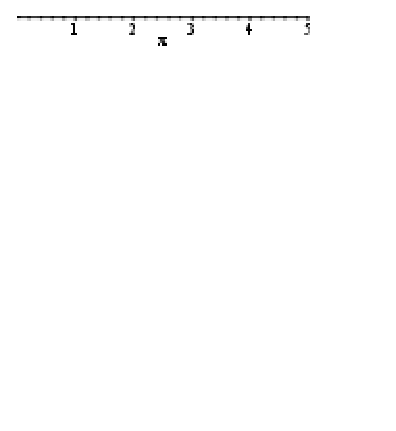
\includegraphics[
height=5.0742cm, width=4.6063cm
]{HJC6Z303.eps} & \FRAME{itbpF}{4.6063cm}{5.0742cm}{0cm}{}{}{Plot}{\special%
{language "Scientific Word";type "MAPLEPLOT";width 4.6063cm;height
5.0742cm;depth 0cm;display "USEDEF";plot_snapshots TRUE;mustRecompute
FALSE;lastEngine "Maple";xmin "-5";xmax "5";xviewmin "0.000000";xviewmax
"5.000000";yviewmin "0.004";yviewmax "1.440650";viewset"XY";plottype
4;numpoints 49;plotstyle "patch";axesstyle "normal";xis \TEXUX{x};yis
\TEXUX{y};var1name \TEXUX{$x$};var2name \TEXUX{$y$};function
\TEXUX{$e^{-x}$};linecolor "black";linestyle 1;pointstyle
"point";linethickness 3;lineAttributes "Solid";var1range
"-5,5";num-x-gridlines 49;curveColor "[flat::RGB:0000000000]";curveStyle
"Line";rangeset"X";valid_file "T";tempfilename
'HJIMTF0I.wmf';tempfile-properties "XPR";}}%
\end{tabular}

\item Modelo logar\'{\i}tmico %$y=\frac{1}{m}\ln x\;m\in\rz,\;m\neq0$%
\FRAME{dhF}{3in}{2.0003in}{0pt}{}{}{Plot}{\special{language "Scientific
Word";type "MAPLEPLOT";width 3in;height 2.0003in;depth 0pt;display
"USEDEF";plot_snapshots TRUE;mustRecompute FALSE;lastEngine "Maple";xmin
"-5";xmax "5";xviewmin "1.000000";xviewmax "5.000000";yviewmin
"0.001";yviewmax "2.018052";viewset"XY";plottype 4;numpoints 49;plotstyle
"patch";axesstyle "normal";xis \TEXUX{x};yis \TEXUX{y};var1name
\TEXUX{$x$};var2name \TEXUX{$y$};function \TEXUX{$\log x$};linecolor
"black";linestyle 1;pointstyle "point";linethickness 3;lineAttributes
"Solid";var1range "-5,5";num-x-gridlines 49;curveColor
"[flat::RGB:0000000000]";curveStyle "Line";rangeset"X";valid_file
"T";tempfilename 'HJIMTF0J.wmf';tempfile-properties "XPR";}}

\item Modelo lineal% $y=mx+b\;\;m,b\in\rz,\;m\neq0$%
\FRAME{dhF}{3in}{2.0003in}{0pt}{}{}{Plot}{\special{language "Scientific
Word";type "MAPLEPLOT";width 3in;height 2.0003in;depth 0pt;display
"USEDEF";plot_snapshots TRUE;mustRecompute FALSE;lastEngine "Maple";xmin
"-5";xmax "5";xviewmin "-5.2";xviewmax "5.204";yviewmin "-2.2";yviewmax
"8.204";plottype 4;numpoints 49;plotstyle "patch";axesstyle "normal";xis
\TEXUX{x};yis \TEXUX{y};var1name \TEXUX{$x$};var2name \TEXUX{$y$};function
\TEXUX{$x+3$};linecolor "black";linestyle 1;pointstyle "point";linethickness
3;lineAttributes "Solid";var1range "-5,5";num-x-gridlines 49;curveColor
"[flat::RGB:0000000000]";curveStyle "Line";valid_file "T";tempfilename
'HJIMTF0K.wmf';tempfile-properties "XPR";}}

\item Modelo polinomico\FRAME{dtbpFUX}{3in}{2.0003in}{0pt}{\Qcb{$%
y=A_{n}x^{n}+A_{n-1}x^{n-1}+\cdots +A_{1}x+A_{0}$}}{}{Plot}{\special%
{language "Scientific Word";type "MAPLEPLOT";width 3in;height 2.0003in;depth
0pt;display "USEDEF";plot_snapshots TRUE;mustRecompute FALSE;lastEngine
"Maple";xmin "-5";xmax "5";xviewmin "-5.2";xviewmax "5.204";yviewmin
"-105.2";yviewmax "165.304";plottype 4;numpoints 49;plotstyle
"patch";axesstyle "normal";xis \TEXUX{x};yis \TEXUX{y};var1name
\TEXUX{$x$};var2name \TEXUX{$y$};function
\TEXUX{$x^{3}+x^{2}+x+5$};linecolor "black";linestyle 1;pointstyle
"point";linethickness 3;lineAttributes "Solid";var1range
"-5,5";num-x-gridlines 49;curveColor "[flat::RGB:0000000000]";curveStyle
"Line";valid_file "T";tempfilename 'HJIMTF0L.wmf';tempfile-properties "XPR";}%
}
\end{enumerate}

\subsection{Ajuste de la curva}

Al observar las gr\'{a}ficas notamos que muchas se parecen y a veces es d%
\'{\i}ficil estar seguro si el modelo que escogemos es adecuado, es m\'{a}s
no conocemos todos los modelos. en esta secci\'{o}n explicaremos dos m\'{e}%
todos para ayudarnos a escoger un modelo que se aproxime de buena forma a
los datos.

\begin{enumerate}
\item Linealizaci\'{o}n :\newline
Este m\'{e}todo consiste en encontrar dos relaciones $h\left( y\right) $ y $%
f\left( x\right) $ tales que al graficar $h\left( y\right) $ vs $f\left(
x\right) $ se obtenga una linea recta, es decir si esto sucede el modelo es
satisfactorio.\newline
Por ejemplo si tenemos los datos 
\begin{equation*}
\begin{tabular}{|l|l|l|l|l|l|}
\hline
$y\left( cm\right) $ & 1 & 4 & 9 & 16 & 25 \\ \hline
$x(s)$ & 1 & 2 & 3 & 4 & 5 \\ \hline
\end{tabular}%
\end{equation*}
\FRAME{dhF}{2.4111in}{1.8343in}{0pt}{}{}{potencial.wmf}{\special{ language
"Scientific Word"; type "GRAPHIC"; maintain-aspect-ratio TRUE; display
"PICT"; valid_file "F"; width 2.4111in; height 1.8343in; depth 0pt;
original-width 3.0415in; original-height 2.3056in; cropleft "0"; croptop
"1"; cropright "1"; cropbottom "0"; filename
'D:/Tacho/potencial.WMF';file-properties "NPEU";}}De acuerdo con la forma el
modelo es $y=ax^{m}$, pero si analizamos los datos ellos nos hacen sospechar
que $m=2,$ por lo que podr\'{\i}amos hacer $h\left( y\right) =y$ y $f\left(
x\right) =x^{2}$ de lo que obtenemos la siguiente tabla 
\begin{equation*}
\begin{tabular}{llllll}
$h\left( y\right) $ & 1 & 4 & 9 & 16 & 25 \\ 
$f\left( x\right) $ & 1 & 4 & 9 & 16 & 25%
\end{tabular}%
\end{equation*}
\FRAME{dhF}{3.3088in}{2.2762in}{0pt}{}{}{cuadra.wmf}{\special{ language
"Scientific Word"; type "GRAPHIC"; maintain-aspect-ratio TRUE; display
"PICT"; valid_file "F"; width 3.3088in; height 2.2762in; depth 0pt;
original-width 3.2638in; original-height 2.2364in; cropleft "0"; croptop
"1"; cropright "1"; cropbottom "0"; filename
'D:/Tacho/cuadra.WMF';file-properties "NPEU";}}Como se obtuvo una recta
podemos decir que el modelo es aceptable y al determinar la ecuaci\'{o}n de
la recta nos que al tomar dos puntos cualesquiera 
\begin{equation*}
a=\frac{y_{1}-y_{2}}{x_{1}^{2}-x_{2}^{2}}=\frac{16-9}{16-9}=1
\end{equation*}
como la relaci\'{o}n matem\'{a}tica es $h\left( y\right) =af\left( x\right)
, $ entonces queda $y=x^{2}.$\newline
Este m\'{e}todo no es pr\'{a}ctico en el sentido de que si no sospechamos
nada acerca de la relaci\'{o}matem\'{a}tica es casi imposible determinar $%
h\left( y\right) $ y $f\left( x\right) ,$ afortunadamente para los modelos
planteados ya existen estas relaciones

\begin{enumerate}
\item Para el modelo $y=ax^{m}$ son 
\begin{equation*}
h\left( y\right) =\log y,\;f\left( x\right) =\log x
\end{equation*}
al obtener la recta \FRAME{dtbpFU}{3.435in}{2.2485in}{0pt}{\Qcb{$\log
Y=m\log x+b,a=10^{b}$}}{}{loglog.wmf}{\special{ language "Scientific Word";
type "GRAPHIC"; maintain-aspect-ratio TRUE; display "PICT"; valid_file "F";
width 3.435in; height 2.2485in; depth 0pt; original-width 3.3892in;
original-height 2.2087in; cropleft "0"; croptop "1"; cropright "1";
cropbottom "0"; filename 'D:/Tacho/loglog.WMF';file-properties "NPEU";}}%
podemos encontrar 
\begin{align*}
m & =\frac{\log y_{i}-\log y_{j}}{\log x_{i}-\log x_{j}} \\
a & =\frac{y_{i}}{x_{i}^{m}}.
\end{align*}
En la pr\'{a}ctica debido a los errores al tomar diferentes parejas $\left(
x_{i},y_{i}\right) $ los valores de $m$ y $a$ no son constantes, por lo que
hay que determinarlos varias veces y promediar los resultados, as\'{\i} la
relaci\'{o}n matem\'{a}tica queda $y=\bar{a}x^{\bar{m}}$

\item Para el modelo $y=ae^{mx}$ se escogen las relaciones 
\begin{equation*}
h\left( y\right) =\ln y,\;f\left( x\right) =x
\end{equation*}
y si obtenemos la recta \FRAME{dhFU}{3.435in}{2.2485in}{0pt}{\Qcb{$\ln
Y=mX+b;\;a=e^{b}$}}{}{semilog.wmf}{\special{ language "Scientific Word";
type "GRAPHIC"; maintain-aspect-ratio TRUE; display "PICT"; valid_file "F";
width 3.435in; height 2.2485in; depth 0pt; original-width 3.3892in;
original-height 2.2087in; cropleft "0"; croptop "1"; cropright "1";
cropbottom "0"; filename 'D:/Tacho/semilog.WMF';file-properties "NPEU";}}%
podemos utilizar 
\begin{align*}
m & =\frac{\ln y_{i}-\ln y_{j}}{x_{i}-x_{j}} \\
a & =\frac{y_{i}}{e^{mx_{i}}}.
\end{align*}
y calculamos varios valores de $m$ y $a$ para promediarlos y obtener la
relaci\'{o}n matem\'{a}tica $y=\bar{a}e^{\bar{m}x}$

\item Si el modelo es $y=\frac{1}{m}\ln x$ las relaciones son 
\begin{equation*}
h\left( y\right) =y,\;f\left( x\right) =\ln x
\end{equation*}
si la gr\'{a}fica $f\left( x\right) \;vs\;h\left( y\right) $ es lineal como
se muestra en la figura \FRAME{dhF}{2.6593in}{1.8334in}{0pt}{}{}{logm.wmf}{%
\special{ language "Scientific Word"; type "GRAPHIC"; maintain-aspect-ratio
TRUE; display "PICT"; valid_file "F"; width 2.6593in; height 1.8334in; depth
0pt; original-width 6.1531in; original-height 4.222in; cropleft "0"; croptop
"1"; cropright "1"; cropbottom "0"; filename
'D:/Tacho/logm.WMF';file-properties "NPEU";}}podemos usar 
\begin{equation*}
m=\frac{\ln x_{i}-\ln x_{j}}{y_{i}-y_{j}}
\end{equation*}
calculamos $m$ varias veces y obtenemos $y=\frac{1}{\bar{m}}\ln x.$

\item El modelo lineal es trivial por lo que dejamos de tarea al lector 
%\end{enumerate}

\item Usando Data Studio es f\'{a}cil realizar el ajuste \newline
Se seleciona la regi\'{o}n de la curva que nos intersa y lugego escogemos en
la barra de herramienta fit y se escoge el modelo adecuado de acuerdcon los
siguientes par\'{a}metros:\FRAME{fhF}{0.6356in}{1.0326in}{0pt}{}{}{ajuste.jpg%
}{\special{ language "Scientific Word"; type "GRAPHIC";
maintain-aspect-ratio TRUE; display "USEDEF"; valid_file "F"; width
0.6356in; height 1.0326in; depth 0pt; original-width 0.6045in;
original-height 0.9997in; cropleft "0"; croptop "1"; cropright "1";
cropbottom "0"; filename 'ajuste.jpg';file-properties "XNPEU";}}

\begin{enumerate}
\item Si se escoge el modelo lineal obtenemos un display parecido al de la
figura\FRAME{dhF}{1.8922in}{1.0326in}{0pt}{}{}{ajuste1.jpg}{\special{
language "Scientific Word"; type "GRAPHIC"; maintain-aspect-ratio TRUE;
display "USEDEF"; valid_file "F"; width 1.8922in; height 1.0326in; depth
0pt; original-width 1.8542in; original-height 0.9997in; cropleft "0";
croptop "1"; cropright "1"; cropbottom "0"; filename
'ajuste1.jpg';file-properties "XNPEU";}}y se dice que el modelo es bueno si $%
r^{2}>0.95$

\item Si se escoge otro modelo obtendremos un display como\FRAME{dbhF}{%
2.0807in}{1.2107in}{0pt}{}{}{ajuste2.jpg}{\special{ language "Scientific
Word"; type "GRAPHIC"; maintain-aspect-ratio TRUE; display "USEDEF";
valid_file "F"; width 2.0807in; height 1.2107in; depth 0pt; original-width
2.0418in; original-height 1.177in; cropleft "0"; croptop "1"; cropright "1";
cropbottom "0"; filename 'ajuste2.jpg';file-properties "XNPEU";}}y decimos
que el modelo es bueno si el mean Square Error es despreciable comparado con 
$\bar{y}$ %\end{enumerate}

\item Ajuste lineal\newline
El ajuste lineal es un m\'{e}todo estad\'{\i}stico, parecido al anterior,
pero usando herramientas diferentes.\newline
En este caso no explicaremos mucho , s\'{o}lo plantearemos algunas f\'{o}%
rmulas e interpretaremos los resultados \newline
Si tenemos dos conjuntos de datos 
\begin{align*}
& x_{1},x_{2},x_{3},\cdots,x_{n} \\
& y_{1},y_{2},y_{3},\cdots,y_{n}
\end{align*}
definiremos la

\begin{enumerate}
\item Media aritm\'{e}tica 
\begin{align*}
\bar{x} & =\frac{\sum_{i=1}^{n}x_{i}}{n} \\
\bar{y} & =\frac{\sum_{i=1}^{n}y_{i}}{n}
\end{align*}

\item Varianza 
\begin{align*}
S_{xx}^{2} & =\frac{\sum_{i=1}^{n}(x_{i}-\bar{x})^{2}}{n-1} \\
S_{yy}^{2} & =\frac{\sum_{i=1}^{n}(y_{i}-\bar{y})^{2}}{n-1}
\end{align*}

\item Covarianza 
\begin{equation*}
S_{xy}=\frac{\sum_{i=1}^{n}(x_{i}-\bar{x})(y_{i}-\bar{y})}{n-1}
\end{equation*}

\item Coeficiente de correlaci\'{o}n 
\begin{equation*}
r=\frac{S_{xy}}{\sqrt{S_{xx}^{2}S_{yy}^{2}}}
\end{equation*}
Cuando estudiamos dos variables $X\;$y $Y$, en realidad estas variables
estas variables tienen desde el punto de vista geom\'{e}trico el
comportamiento de dos vectores (rayos con direcci\'{o}n). Y se dice que
existe un ajuste lineal si los vectores representados por las desviaciones
est\'{a}n alineados o son paralelos.\newline
Para determinar si esto sucede podemos utilizar la trigonometr\'{\i}a para
determinar el \'{a}ngulo entre los vectores representados en la figura 
\FRAME{dhF}{1.8152in}{1.4659in}{0pt}{}{}{veca.wmf}{\special{ language
"Scientific Word"; type "GRAPHIC"; maintain-aspect-ratio TRUE; display
"PICT"; valid_file "F"; width 1.8152in; height 1.4659in; depth 0pt;
original-width 1.7781in; original-height 1.4304in; cropleft "0"; croptop
"1"; cropright "1"; cropbottom "0"; filename
'D:/Tacho/veca.WMF';file-properties "NPEU";}}
\end{enumerate}

%\end{enumerate}
Utilizando una rama de las matem\'{a}ticas llamada algebra lineal se puede
comprobar que si $\theta$ es el \'{a}ngulo entre los vectores entonces 
\begin{equation*}
\cos\theta=r
\end{equation*}
Es decir este coeficiente determina la relaci\'{o}n lineal entre las
desviaciones de las variables y esta dependencia es perfecta cuando $r=\pm1$
existe el ajuste lineal en la practica esto no sucede debido a los errores
pero decimos que el ajuste es aceptable si $r^{2}>0.95.\;$\newline
Si el ajuste existe deben existir dos relaciones $h\left( y\right) $ y $%
f\left( x\right) $ tal que el modelo 
\begin{equation*}
h\left( y\right) =mf\left( x\right) +b
\end{equation*}
debe tener un $r$ adecuado \ y se puede calcular 
\begin{equation*}
r=\frac{n\sum_{i.j=1}^{n}f\left( x_{i}\right) h\left( y_{j}\right)
-\sum_{i=1}^{n}f\left( x_{i}\right) \sum_{j=1}^{n}h\left( y_{i}\right) }{%
\sqrt{\left[ n\sum_{i=1}^{n}f^{2}\left( x_{i}\right) -\left( \sum
_{i=1}^{2}f\left( x_{i}\right) ^{2}\right) \right] }\left[ n\sum
_{j=1}^{n}h^{2}\left( y_{j}\right) -\left( \sum_{j=1}^{2}h\left(
y_{j}\right) ^{2}\right) \right] }
\end{equation*}
\begin{align*}
m & =\frac{n\sum_{i.j=1}^{n}f\left( x_{i}\right) h\left( y_{j}\right)
-\sum_{i=1}^{n}f\left( x_{i}\right) \sum_{j=1}^{n}h\left( y_{i}\right) }{%
n\sum_{i=1}^{n}f^{2}\left( x_{i}\right) -\left( \sum_{i=1}^{2}f\left(
x_{i}\right) ^{2}\right) } \\
b & =\frac{\sum_{j=1}^{n}h\left( y_{j}\right) -m\sum_{i=1}^{n}f\left(
x_{i}\right) }{n}
\end{align*}
donde \ $a$ se obtiene

\begin{itemize}
\item $a=10^{b}$ en el modelo $y=ax^{m}$

\item $a=e^{b}$ en el modelo $y=ae^{mx}$
\end{itemize}

Interpretaci\'{o}n geom\'{e}trica de la covarianza

Si consideramos una nube de puntos formados por las parejas de los datos
concretos de dos variables $X$ e $Y$ $\left( x_{i},y_{i}\right) $ el centro
de gravedad de esta nube de puntos es $\left( \overset{-}{x},\overset{-}{y}%
\right) $, ahora si trasladamos los ejes de tal forma que este punto sea el
centro, la nube queda dividida en cuatro cuadrantes los que indica que los
puntos que se encuentran en el pimer y tercer cuadrante contribuyen
positivamente al valor de la covarianza y los que se encuentran en los otros
dos cuadrantes contribuyen negativamente. como lo indica la figura.a y si
los puntos se reparten con igual proporci\'{o}n la covarianza ser\'{a}
negativa como indica la segunda gr\'{a}fica de la figura a\FRAME{ftbpFU}{%
3.0528in}{1.817in}{0pt}{\Qcb{fig a}}{}{fig4.wmf}{\special{language
"Scientific Word";type "GRAPHIC";maintain-aspect-ratio TRUE;display
"USEDEF";valid_file "F";width 3.0528in;height 1.817in;depth
0pt;original-width 5.6351in;original-height 3.333in;cropleft "0";croptop
"1";cropright "1";cropbottom "0";filename
'D:/Tacho/fig4.wmf';file-properties "NPEU";}}y no hay relaci\'{o}n matem\'{a}%
tica si la nube de puntos no tiene ninguna tendencia como en la fig b\FRAME{%
dhFU}{2.7743in}{1.817in}{0pt}{\Qcb{fig b}}{}{fig4cb.wmf}{\special{language
"Scientific Word";type "GRAPHIC";maintain-aspect-ratio TRUE;display
"USEDEF";valid_file "F";width 2.7743in;height 1.817in;depth
0pt;original-width 5.6455in;original-height 3.6772in;cropleft "0";croptop
"1";cropright "1";cropbottom "0";filename
'D:/Tacho/fig4cb.wmf';file-properties "NPEU";}}%
%\end{document}
\end{enumerate}
\end{enumerate}
\end{enumerate}

\section{About This Shell}

This shell document provides a sample layout of a Standard LaTeX Article.

The front matter has a number of sample entries that you should replace with
your own. Replace this text with your own. You may delete all of the text in
this document to start with a blank document.

Changes to the typeset format of this shell and its associated \LaTeX{}
formatting file (\texttt{article.cls}) are not supported by MacKichan
Software, Inc. If you wish to make such changes, please consult the \LaTeX{}
manuals or a local \LaTeX{} expert.

If you modify this document and save it as ``Standard LaTeX Article.shl'' in
the \texttt{Shells\TEXTsymbol{\backslash}Articles\TEXTsymbol{\backslash}SW}
directory, it will become your new Standard LaTeX Article shell.

The typesetting specification selected by this shell document uses the
default class options. There are a number of class options supported by this
typesetting specification. The available options include setting the paper
size and the point size of the font used in the body of the document. Select 
\textsf{Typeset, Options and Packages}, the \textsf{Class Options} tab and
then click the \textsf{Modify} button to see the class options that are
available for this typesetting specification.

\section{Features of This Shell}

\subsection{Subsection}

Use the Section tag for major sections, and the Subsection tag for
subsections.

\subsubsection{Subsubsection}

This is just some harmless text under a subsubsection.

\paragraph{Subsubsubsection}

This is just some harmless text under a subsubsubsection.

\subparagraph{Subsubsubsubsection}

This is just some harmless text under a subsubsubsubsection.

\subsection{Tags}

You can apply the logical markup tag \emph{Emphasized}.

You can apply the visual markup tags \textbf{Bold}, \textit{Italics}, 
\textrm{Roman}, \textsf{Sans Serif}, \textsl{Slanted}, \textsc{Small Caps},
and \texttt{Typewriter}.

You can apply the special, mathematics only, tags $\mathbb{BLACKBOARD}$ $%
\mathbb{BOLD}$, $\mathcal{CALLIGRAPHIC}$, and $\mathfrak{fraktur}$. Note
that blackboard bold and calligraphic are correct only when applied to
uppercase letters A through Z.

You can apply the size tags {\tiny tiny}, {\scriptsize scriptsize}, 
{\footnotesize footnotesize}, {\small small}, {\normalsize normalsize}, 
{\large large}, {\Large Large}, {\LARGE LARGE}, {\huge huge} and {\Huge Huge}%
.

\QTP{Body Math}
This is a Body Math paragraph. Each time you press the Enter key, Scientific
WorkPlace switches to mathematics mode. This is convenient for carrying out
``scratchpad'' computations.

Following is a group of paragraphs marked as Body Quote. This environment is
appropriate for a short quotation or a sequence of short quotations.

\begin{quote}
The buck stops here. \emph{Harry Truman}

Ask not what your country can do for you; ask what you can do for your
country. \emph{John F Kennedy}

I am not a crook. \emph{Richard Nixon}

It's no exaggeration to say the undecideds could go one way or another. 
\emph{George Bush}

I did not have sexual relations with that woman, Miss Lewinsky. \emph{Bill
Clinton}
\end{quote}

The Quotation tag is used for quotations of more than one paragraph. \
Following is the beginning of \emph{Alice's Adventures in Wonderland }by
Lewis Carroll:

\begin{quotation}
Alice was beginning to get very tired of sitting by her sister on the bank,
and of having nothing to do: once or twice she had peeped into the book her
sister was reading, but it had no pictures or conversations in it, 'and what
is the use of a book,' thought Alice 'without pictures or conversation?'

So she was considering in her own mind (as well as she could, for the hot
day made her feel very sleepy and stupid), whether the pleasure of making a
daisy-chain would be worth the trouble of getting up and picking the
daisies, when suddenly a White Rabbit with pink eyes ran close by her.

There was nothing so very remarkable in that; nor did Alice think it so very
much out of the way to hear the Rabbit say to itself, 'Oh dear! Oh dear! I
shall be late!' (when she thought it over afterwards, it occurred to her
that she ought to have wondered at this, but at the time it all seemed quite
natural); but when the Rabbit actually took a watch out of its
waistcoat-pocket, and looked at it, and then hurried on, Alice started to
her feet, for it flashed across her mind that she had never before seen a
rabbit with either a waistcoat-pocket, or a watch to take out of it, and
burning with curiosity, she ran across the field after it, and fortunately
was just in time to see it pop down a large rabbit-hole under the hedge.

In another moment down went Alice after it, never once considering how in
the world she was to get out again.
\end{quotation}

Use the Verbatim tag when you want \LaTeX{} to preserve spacing, perhaps
when including a fragment from a program such as:
\begin{verbatim}
#include <iostream>        // < > is used for standard libraries.
void main(void)            // ''main'' method always called first.
{
  cout << ''Hello World.'';  // Send to output stream.
}
\end{verbatim}

\subsection{Mathematics and Text}

Let $H$ be a Hilbert space, $C$ be a closed bounded convex subset of $H$, $T$
a nonexpansive self map of $C$. Suppose that as $n\rightarrow \infty $, $%
a_{n,k}\rightarrow 0$ for each $k$, and $\gamma _{n}=\sum_{k=0}^{\infty
}\left( a_{n,k+1}-a_{n,k}\right) ^{+}\rightarrow 0.$ Then for each $x$ in $C$%
, $A_{n}x=\sum_{k=0}^{\infty }a_{n,k}T^{k}x$ converges weakly to a fixed
point of $T$ .

The numbered equation 
\begin{equation}
u_{tt}-\Delta u+u^{5}+u\left| u\right| ^{p-2}=0\text{ in }\mathbf{R}%
^{3}\times \left[ 0,\infty \right[ .  \label{eqn1}
\end{equation}
is automatically numbered as equation \ref{eqn1}.

\subsection{List Environments}

You can create numbered, bulleted, and description lists using the tag popup
at the bottom left of the screen.

\begin{enumerate}
\item List item 1

\item List item 2

\begin{enumerate}
\item A list item under a list item.

The typeset style for this level is different than the screen style. \ The
screen shows a lower case alphabetic character followed by a period while
the typeset style uses a lower case alphabetic character surrounded by
parentheses.

\item Just another list item under a list item.

\begin{enumerate}
\item Third level list item under a list item.

\begin{enumerate}
\item Fourth and final level of list items allowed.
\end{enumerate}
\end{enumerate}
\end{enumerate}
\end{enumerate}

\begin{itemize}
\item Bullet item 1

\item Bullet item 2

\begin{itemize}
\item Second level bullet item.

\begin{itemize}
\item Third level bullet item.

\begin{itemize}
\item Fourth (and final) level bullet item.
\end{itemize}
\end{itemize}
\end{itemize}
\end{itemize}

\begin{description}
\item[Description List] Each description list item has a term followed by
the description of that term. Double click the term box to enter the term,
or to change it.

\item[Bunyip] Mythical beast of Australian Aboriginal legends.
\end{description}

\subsection{Theorem-like Environments}

The following theorem-like environments (in alphabetical order) are
available in this style.

\begin{acknowledgement}
This is an acknowledgement
\end{acknowledgement}

\begin{algorithm}
This is an algorithm
\end{algorithm}

\begin{axiom}
This is an axiom
\end{axiom}

\begin{case}
This is a case
\end{case}

\begin{claim}
This is a claim
\end{claim}

\begin{conclusion}
This is a conclusion
\end{conclusion}

\begin{condition}
This is a condition
\end{condition}

\begin{conjecture}
This is a conjecture
\end{conjecture}

\begin{corollary}
This is a corollary
\end{corollary}

\begin{criterion}
This is a criterion
\end{criterion}

\begin{definition}
This is a definition
\end{definition}

\begin{example}
This is an example
\end{example}

\begin{exercise}
This is an exercise
\end{exercise}

\begin{lemma}
This is a lemma
\end{lemma}

\begin{proof}
This is the proof of the lemma.
\end{proof}

\begin{notation}
This is notation
\end{notation}

\begin{problem}
This is a problem
\end{problem}

\begin{proposition}
This is a proposition
\end{proposition}

\begin{remark}
This is a remark
\end{remark}

\begin{solution}
This is a solution
\end{solution}

\begin{summary}
This is a summary
\end{summary}

\begin{theorem}
This is a theorem
\end{theorem}

\begin{proof}[Proof of the Main Theorem]
This is the proof.
\end{proof}

\appendix

\section{The First Appendix}

The appendix fragment is used only once. Subsequent appendices can be
created using the Section Section/Body Tag.

\end{document}
